\documentclass{beamer}
\usepackage{etex}
\usetheme{Antibes}
\usepackage{amssymb,amsmath,amsthm}
\usepackage{graphicx}
\usepackage{caption}
\usepackage{subfig}
%\definecolor{cardinal}{rgb}{0.77, 0.12, 0.23}
%\usecolortheme[named=cardinal]{structure}
%\setbeamercolor{block title}{bg=cardinal,fg=black}
 \usepackage{tikz}
 \usetikzlibrary{patterns,snakes,plotmarks}
 \usepackage{multirow}
% \usetikzlibrary{shadows}
\usepackage{epstopdf}
\usepackage{nicefrac}
\usepackage{lmodern}
\usepackage{pgfplots}
\usepackage{qtree}
\newcommand*{\Scale}[2][4]{\scalebox{#1}{\ensuremath{#2}}}%
\DeclareCaptionLabelSeparator{horse}{:\,\,} % change according to your needs
\captionsetup{
  labelsep = horse,
  figureposition = bottom % used to get the correct vertical space between the figure and the caption
}
\setbeamertemplate{caption}[numbered]
\setbeamertemplate{items}[circle]
\setbeamertemplate{enumerate items}[square]
\theoremstyle{definition}
\newtheorem*{exs}{Examples}
\newtheorem{ex}{Example}
\newtheorem*{exc}{Exercise}
\newcommand{\bn}{\begin{enumerate}[i)]}
\newcommand{\en}{\end{enumerate}}
\newcommand{\im}{\item}
\newcommand{\CPT}[1]{\large{\textbf{CHAPTER #1}}}
\newcommand{\ir}[1]{\textbf{Remark #1}}
\newcommand{\ith}[1]{\textbf{Theorem #1}}
\newcommand{\idf}[1]{\textbf{Definition #1}}
\newcommand{\iex}[1]{\textbf{Example #1}}

%\usepackage{booktabs}
\setlength{\parindent}{0pt}
%\setbeameroption{show notes}
 \setbeamerfont{note page}{size=\tiny}
%\setbeamertemplate{note page}[plain]
%\setbeameroption{show only notes}
\title{Math 629 - Survival Analysis \\ Chapter 1}
\author{Drew Lazar}
\institute{Ball State University}
\date{\today}

\begin{document}
\begin{frame}
    \titlepage
\end{frame}
\section{Chapter 1} 
\begin{frame}\frametitle{Types of Censoring}
\bn
\item \textbf{Right Censoring:} An observation is \textbf{right censored} if the survival time is longer than its observed value. Some examples:
\bni
\item A five year study is conducted on how long it takes for machines to break down. A particular machine is observed from the start of the study but breaks down \textbf{after the study ends}.
\item Patients are followed for ten years after having a major heart attack. The response variable is time until death. A patient \textbf{withdraws} from the study after being followed for 2 years and moves to another country.
\item A study is done on smokers who have quit to see if they will resume smoking. Study participants are contacted by telephone. A participant changes his phone number, can not be reached and is \textbf{lost to follow-up}.
\en
\en
\end{frame}
\begin{frame} \frametitle{Types of Censoring cont'd}

\bn \setcounter{enumi}{2}
\item \textbf{Left Censoring:} An observation is \textbf{left censored} if the survival time is shorter than its observed value. For example, we following persons at risk until they become HIV positive.  For some patients we may not know the exact time becoming HIV, and therefore do not know exactly when the failure occurred.
\item \textbf{Interval Censoring:} An observation is \textbf{interval censored} if the event is known to occur in some interval. For example, a study is done to see the time until children can count to ten. The children are observed every 2 months. A child can count to ten at a follow-up time but couldn't count to ten at the previous visit.
\en
\end{frame}


\begin{frame}
\begin{columns}
    \begin{column}{0.48\textwidth}
        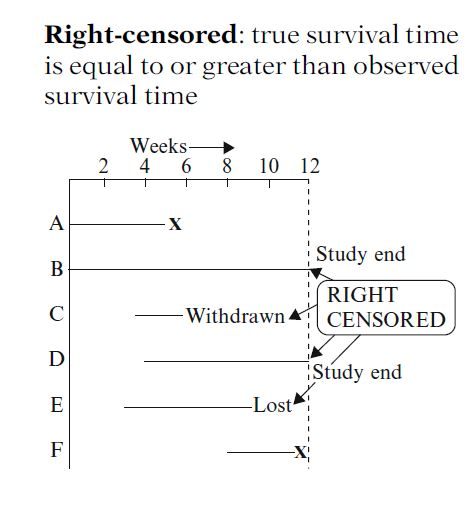
\includegraphics[width = \textwidth]{Ch1-RightCensor.JPG}
    \end{column}
    \hspace{-40pt}
    \begin{column}{0.48\textwidth}
         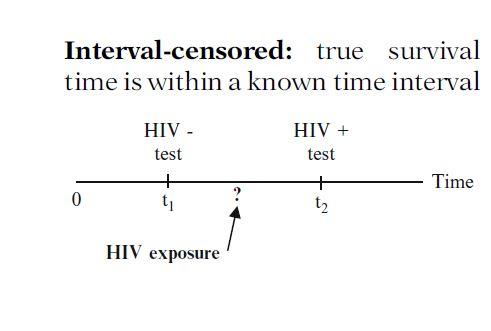
\includegraphics[width = \textwidth]{Ch1-IntervalCensor.JPG} \\
              \vspace{-20pt}
         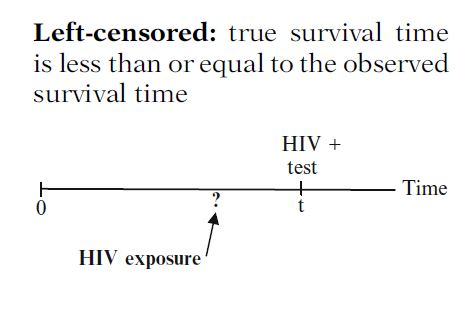
\includegraphics[width =\textwidth]{Ch1-LeftCensor.JPG}
    \end{column}
\end{columns}
\end{frame}
\section{Chapter 2} 
\begin{frame}
\begin{block}{Problem 2.1}
Given the data below use R to create Kaplan-Kaplan Meirer curves. 
\end{block}  
\end{frame} 

\end{document} 